\section{Layers of the Reference Architecture Model}\label{sec:layers}
The five layers of the Reference Architecture Model are presented in detail in the following subsections.

\subsection{Business Layer}\label{subsec:business_layer}
%\addcontentsline{toc}{subsection}{Business Layer}
The Business Layer of the Reference Architecture Model defines and categorizes the different roles the participants in the International Data Spaces may assume. Furthermore, it specifies basic patterns of interaction taking place between these roles. It thereby contributes to the development of innovative business models and digital, data-driven services to be used by the participants in the International Data Spaces. 

While the Business Layer provides an abstract description of the roles in the International Data Spaces, it can be considered a blueprint for the other, more technical layers. The Business Layer can therefore be used to verify the technical architecture of the International Data Spaces. In this sense, the Business Layer specifies the requirements to be addressed by the Functional Layer (see section \ref{sec_functional_layer}). 

%ToDo:update subsection
\subsubsection{Roles in the International Data Spaces}
%\addcontentsline{toc}{subsubsection}{Roles in the International Data Spaces}
In the following, each role a participant can assume in the International Data Spaces is described in detail, together with the basic tasks assigned to it. The majority of roles require certification of the organization that wants to assume that role, including certification of the technical, physical, and organizational security mechanisms the organization employs. Certification of organizations that want to participate in the International Data Spaces is considered a fundamental measure to establish trust among all participants (especially with regard to roles that are crucial for the overall functioning of the International Data Spaces, such as the Broker Service Provider, the App Store Provider, the Identity Provider, or the Clearing House). The Certification Scheme applied in the participant evaluation process is described in detail in Section 4.2.
%ToDo: refer to sec 4.2

There are four categories of roles:

\begin{itemize}
	\item Category 1: Core Participant

	\item Category 2: Intermediary

	\item Category 3: Software / Service Provider

	\item Category 4: Governance Body
\end{itemize}\par



\paragraph{Category 1: Core Participant}
Core Participants are involved and required every time data is exchanged in the International Data Spaces. Roles assigned to this category are Data Owner, Data Provider, Data Consumer, Data User, and App Provider. The role of a Core Participant can be assumed by any organization that owns, wants to provide, and/or wants to consume or use data.
\todo{CQ: Wie/Warum ist der App Provider hier reingekommen? Der ist doch für einen Datenaustausch nicht notwendig}

Benefit for participants in the International Data Spaces is created by these roles as they make data available (Data Owner), provide data (Data Provider), or consume/use data (Data Consumer, Data User, App Provider). In addition, Data Providers and Data Consumers may apply business models (including pricing models) as deemed appropriate.

\paragraph{Data Owner} %ToDo: refer to section 4.3.4
As the legal situation regarding data ownership is very complicated (as discussed in section 4.3.4), the term ‘Data Owner’ is not used in a legal understanding in this document. The Reference Architecture Model takes an operational data management perspective, defining a Data Owner as a legal entity or natural person creating data and/or executing control over it. This enables the Data Owner to define Data Usage Policies and provide access to its data. Data Ownership includes at least two major concepts:

\begin{itemize}
	\item having the (technical) means and the responsibility to define Usage Contracts and Usage Policies, and to provide access to data; and 

	\item having the (technical) means and the responsibility to define the Payment Model, including the model for reuse of data by third parties. 
\end{itemize}

Usually, a participant acting as Data Owner automatically assumes the role of the Data Provider as well. However, there may be cases in which the Data Provider is not the Data Owner (e.g., if the data is technically managed by a different entity than the Data Owner, such as in the case of a company using an external IT service provider for data management, or if data management activities are handed over to a data trustee).

In cases in which the Data Owner does not act as the Data Provider at the same time, the only activity of the Data Owner is to authorize a Data Provider to make its data available to be used by a Data Consumer. Any such authorization should be documented by a contract, which should include data usage policy information for the data provided (see. Section 4.1.3.6). The contract needs not necessarily be a paper document, but may be an electronic file as well.
%ToDo: refer to section 4.1.3.6

\paragraph{Data Provider}
The Data Provider makes data available for being exchanged between a Data Owner and a Data Consumer. As already mentioned above, the Data Provider is in most cases identical with the Data Owner, but not necessarily. To submit metadata to a Broker, or exchange data with a Data Consumer, the Data Provider uses software components that are compliant with the Reference Architecture Model of the International Data Spaces.

Providing a Data Consumer with data from a Data Owner is the main activity of the Data Provider. To facilitate a data request from a Data Consumer, the Data Provider should provide a Broker Service Provider (see below) with proper metadata about the data. However, a Broker Service Provider is not necessarily required for a Data Consumer and a Data Provider to establish a connection.

Exchanging data with a Data Consumer needs not necessarily be the only activity of the Data Provider. At the end of a data exchange transaction completely or partially executed, for example, the Data Provider may log the details of the successful (or unsuccessful) completion of the transaction at a Clearing House (see below) to facilitate billing or resolve a conflict. Furthermore, the Data Provider can use Data Apps to enrich or transform the data in some way, or to improve its quality. (Data Apps are specific applications that can be integrated into the data exchange workflow between two or more participants in the International Data Spaces.)

If the technical infrastructure for participating in the International Data Spaces is not deployed by the Data Consumer, a Data Provider may use a Service Provider (see below) to connect to the International Data Spaces.

\paragraph{Data Consumer}
The Data Consumer receives data from a Data Provider. From a business process modeling perspective, the Data Consumer is the mirror entity of the Data Provider; the activities performed by the Data Consumer are therefore similar to the activities performed by the Data Provider.

Before the connection to a Data Provider can be established, the Data Consumer can search for existing datasets by making an inquiry at a Broker Service Provider. The Broker Service Provider then provides the required metadata for the Data Consumer to connect to a Data Provider. Alternatively, the Data Consumer can establish a connection with a Data Provider directly (i.e., without involving a Broker Service Provider). In cases in which the information to connect with the Data Provider is already known to the Data Consumer, the Data Consumer may request the data (and the corresponding metadata) directly from the Data Provider.

Like a Data Provider, the Data Consumer may log the details of a successful (or unsuccessful) data exchange transaction at a Clearing House, use Data Apps to enrich, transform, etc. the data received, or use a Service Provider to connect to the International Data Spaces (if it does not deploy the technical infrastructure for participation itself).

\paragraph{Data User}
Similar to the Data Owner being the legal entity that has the legal control over its data, the Data User is the legal entity that has the legal right to use the data of a Data Owner as specified by the usage policy. In most cases, the Data User is identical with the Data Consumer. However, there may be scenarios in which these roles are assumed by different participants. For example, a patient could use a web-based software system to manage their personal health data and grant access to this data to a health coach. The data could be received from a hospital. In this case, the health coach would be the Data User and the provider of the web-based software system would be the Data Consumer.

\paragraph{App Provider} %ToDo: Refer to sec 3.5
App Providers develop Data Apps to be used in the International Data Spaces. To be deployable, a Data App has to be compliant with the system architecture of the International Data Spaces (see Section 3.5). In addition, Data Apps can be certified by a Certification Body in order to increase trust in these applications (especially with regard to Data Apps processing sensitive information). Each Data App must be published in the App Store for being accessed and used by Data Consumers and Data Providers. App Providers should describe each Data App using metadata (in compliance with a metadata model) with regard to its semantics, functionality, interfaces, etc.).


\paragraph{Category 2: Intermediary}
Intermediaries act as trusted entities. Roles assigned to this category are Broker Service Provider, Clearing House, Identity Provider, App Store Provider, and Vocabulary Provider. These roles may be assumed only by trusted organizations. 

Benefit for participants in the International Data Spaces is created by these roles by establishing trust, providing metadata, and creating a business model around their services.

\paragraph{Broker Service Provider}
The Broker Service Provider is an intermediary that stores and manages information about the data sources available in the International Data Spaces. As the role of the Broker Service Provider is central but non-exclusive, multiple Broker Service Providers may be around at the same time (e.g., for different application domains). An organization offering broker services in the International Data Spaces may assume other intermediary roles at the same time (e.g., Clearing House or Identity Provider, see below). Nevertheless, it is important to distinguish organizations and roles (e.g., assuming the role of a Broker Service Provider means that an organization deals only with metadata management; at the same time, the same organization may assume the role of a Clearing House, for which completely different tasks are defined).

The activities of the Broker Service Provider mainly focus on receiving and providing metadata. The Broker Service Provider must provide an interface for Data Providers to send their metadata. The metadata should be stored in an internal repository for being queried by Data Consumers in a structured manner. While the core of the metadata model must be specified by the International Data Spaces (i.e., by the Information Model, see Section 3.4), a Broker Service Provider may extend the metadata model to manage additional metadata elements.
%ToDo: refer to sec 3.4

After the Broker Service Provider has provided the Data Consumer with the metadata about a certain Data Provider, its job is done (i.e., it is not involved in the subsequent data exchange process).


\paragraph{Clearing House}
The Clearing House is an intermediary that provides clearing and settlement services for all financial and data exchange transactions. In the International Data Spaces, clearing activities are separated from broker services, since these activities are technically different from maintaining a metadata repository. As already stated above, it might still be possible that the two roles $``$Clearing House$"$  and $``$Broker Service Provider$"$  are assumed by the same organization, as both roles require acting as a trusted intermediary between the Data Provider and the Data Consumer.

The Clearing House logs all activities performed in the course of a data exchange. After a data exchange, or parts of it, has been completed, both the Data Provider and the Data Consumer confirm the data transfer by logging the details of the transaction at the Clearing House. Based on this logging information, the transaction can then be billed. The logging information can also be used to resolve conflicts (e.g., to clarify whether a data package has been received by the Data Consumer or not). The Clearing House also provides reports on the performed (logged) transactions for billing, conflict resolution, etc.

\paragraph{Identity Provider}
The Identity Provider should offer a service to create, maintain, manage, monitor, and validate identity information of and for participants in the International Data Spaces\textit{. }This is imperative for secure operation of the International Data Spaces and to avoid unauthorized access to data. 

The Identity Provider consist of a Certification Authority (managing digital certificates for the participants of the International Data Spaces), a Dynamic Attribute Provisioning Service (DAPS, managing the dynamic attributes of the participants), and a service named Dynamic Trust Monitoring (DTM, for continuous monitoring of the security and behavior of the network. More details about identity management can be found in section 4.1. %ToDo refer to sec 4.1

\paragraph{App Store Provider}
The App Store provides Data Apps. These are applications that can be deployed inside the Connector, the core technical component required for a participant to join the International Data Spaces. Data Apps facilitate data processing workflows. They may be certified by a Certification Body, following the certification procedures defined in Section 4.2. %ToDo: refer to sec 4.2

The App Store is responsible for managing information about Data Apps offered by App Providers (see below). The App Store should provide interfaces for publishing and retrieving Data Apps plus corresponding metadata.

\paragraph{Vocabulary Provider}
The Vocabulary Provider manages and offers vocabularies (i.e., ontologies, reference data models, or metadata elements) that can be used to annotate and describe datasets. In particular, the Vocabulary Provider provides the Information Model of the International Data Spaces, which is the basis for the description of data sources (see Section 3.4). In addition, other domain specific vocabularies can be provided. %ToDo refer

\paragraph{Category 3: Software / Service Provider}
This category comprises IT companies providing software and/or services (e.g., based on a software-as-a-service model) to the participants of the International Data Spaces. Roles subsumed under this category are Service Provider and Software Provider.

Benefit is created by these roles by providing software and services to the participants of the International Data Spaces. 

It should be noted that the process of providing software to be used for establishing the endpoints of a data exchange transaction (e.g. Enterprise Systems like ERP or MES, or other platforms) is not part of the International Data Spaces, as it takes place before an organization joins the IDS.



\paragraph{Service Provider}
If a participant does not deploy the technical infrastructure required for participation in the International Data Spaces itself, it may transfer the data to be made available in the International Data Spaces to a Service Provider hosting the required infrastructure for other organizations.

This role includes also providers offering additional data services (e.g., for data analysis, data integration, data cleansing, or semantic enrichment) to improve the quality of the data exchanged in the International Data Spaces. From a technical point of view, such a Service Provider can be considered a Data Provider and a Data Consumer at the same time (e.g., as a Data Consumer, it receives data from a Data Provider, then provides its specific service, and then turns into a Data Provider itself and offers the data in the International Data Spaces). 

Unlike the services provided by a Service Provider, Data Apps can be installed in the IT environment of a Data Consumer or Data Provider for implementing additional data processing functionality. To use the functionality of a Data App, the data therefore does not have to be transferred to an external Service Provider.

\paragraph{Software Provider}
A Software Provider provides software for implementing the functionality required by the International Data Spaces (i.e., through software components, as described in Section 3.5). Unlike Data Apps, software is not provided by the App Store, but delivered over the Software Providers’ usual distribution channels, and used on the basis of individual agreements between the Software Provider and the user (e.g., a Data Consumer, a Data Provider, or a Broker Service Provider). This procedure implies that the agreements between Software Providers and Data Consumers, Data Providers, etc. remain outside the scope of the International Data Spaces.

\paragraph{Category 4: Governance Body}
The Certification Body, Evaluation Facilities, and the International Data Spaces Association are the Governance Bodies of the International Data Spaces.

Benefit for participants in the International Data Spaces is created by the Certification Body and the Evaluation Facilities by taking care of the certification process and issuing certificates (both with regard to organizations that want to participate and with regard to software components that are to be used).

\paragraph{Certification Body and Evaluation Facilities}
The Certification Body, together with selected Evaluation Facilities, is in charge of the certification of the participants and the core technical components in the International Data Spaces. These Governance Bodies make sure that only compliant organizations are granted access to the trusted business ecosystem.  In this process, the Certification Body supervises the actions and decisions of the Evaluation Facilities. 

The Certification Scheme applied in the process is described in Section 4.2. %ToDO refer to sec 4.2

\paragraph{International Data Spaces Association (IDSA)}
The International Data Spaces Association (IDSA) is a non-profit organization promoting the continuous development of the International Data Spaces. More specifically, it supports and governs the continuous development of the Reference Architecture Model and the participant certification process. The International Data Spaces Association is currently organized across several working groups, each one addressing a specific topic (e.g., architecture, use cases and requirements, or certification). Members of the Association are primarily large industrial enterprises, IT companies, SMEs, research institutions, and industry associations.

As the International Data Spaces Association is not directly involved in the data exchange activities of the International Data Spaces, its role will not be further addressed in the sections on the other Layers.


\subsubsection*{Interaction of Roles }
%\addcontentsline{toc}{subsubsection}{Interaction of Roles }
\paragraph{Basic interactions for data exchange and data sharing in the International Data Spaces}
Figure \ref{fig:_Roles_and_interactions_in_the_International_Data_Spaces} gives an overview of the roles and the interactions taking place between them. As some of the roles (Certification Body and Evaluation Facilities) are not actively involved in the everyday operations of the International Data Spaces, they are omitted from the illustration. Also, the figure does not include Software Providers and Identity Providers, because of the necessary connection of those roles with all other roles. The Software Provider would be connected to all other roles with the relation $``$provides software$"$ . Likewise, the Identity Provider would be connected to all other roles with the relation $``$provides identity$"$ .

Figure \ref{fig:_Roles_and_interactions_in_the_International_Data_Spaces} shows only the basic interactions taking place between the different roles in the International Data Spaces. For data exchange, additional, more specific interactions are necessary. These interactions are described in the Process Layer section of the Reference Architecture Model (see section 3.3). %ToDo: refer to sec 3.3.

Table \ref{tab:interactions} gives an overview of possible (mandatory or optional) interactions taking place in the IDS. 



%%%%%%%%%%%%%%%%%%%% Table No: 2 starts here %%%%%%%%%%%%%%%%%%%%


\begin{table}[H]
 			\centering
\begin{tabular}{p{1.03in}p{0.22in}p{0.22in}p{0.22in}p{0.13in}p{0.13in}p{0.22in}p{0.59in}p{0.22in}p{0.2in}p{0.2in}p{0.13in}p{0.06in}p{0.13in}}
\hline
%row no:1
\multicolumn{1}{|p{1.03in}}{\cellcolor[HTML]{EFEFEF}} & 
\multicolumn{1}{|p{0.22in}}{\cellcolor[HTML]{EFEFEF}{\fontsize{9pt}{10.8pt}\selectfont \textbf{Data Owner}}} & 
\multicolumn{1}{|p{0.22in}}{\cellcolor[HTML]{EFEFEF}{\fontsize{9pt}{10.8pt}\selectfont \textbf{Data Provider}}} & 
\multicolumn{1}{|p{0.22in}}{\cellcolor[HTML]{EFEFEF}{\fontsize{9pt}{10.8pt}\selectfont \textbf{Data consumer}}} & 
\multicolumn{1}{|p{0.13in}}{\cellcolor[HTML]{EFEFEF}{\fontsize{9pt}{10.8pt}\selectfont \textbf{Data User}}} & 
\multicolumn{1}{|p{0.13in}}{\cellcolor[HTML]{EFEFEF}{\fontsize{9pt}{10.8pt}\selectfont \textbf{Broker}}} & 
\multicolumn{1}{|p{0.22in}}{\cellcolor[HTML]{EFEFEF}{\fontsize{9pt}{10.8pt}\selectfont \textbf{Clearing House}}} & 
\multicolumn{1}{|p{0.59in}}{\cellcolor[HTML]{EFEFEF}{\fontsize{9pt}{10.8pt}\selectfont \textbf{Identity Provider}}} & 
\multicolumn{1}{|p{0.22in}}{\cellcolor[HTML]{EFEFEF}{\fontsize{9pt}{10.8pt}\selectfont \textbf{Service Provider}}} & 
\multicolumn{1}{|p{0.2in}}{\cellcolor[HTML]{EFEFEF}{\fontsize{9pt}{10.8pt}\selectfont \textbf{App Provider}}} & 
\multicolumn{1}{|p{0.2in}}{\cellcolor[HTML]{EFEFEF}{\fontsize{9pt}{10.8pt}\selectfont \textbf{App Store Provider}}} & 
\multicolumn{1}{|p{0.13in}}{\cellcolor[HTML]{EFEFEF}{\fontsize{9pt}{10.8pt}\selectfont \textbf{Vocabulary Provider}}} & 
\multicolumn{1}{|p{0.06in}}{\cellcolor[HTML]{EFEFEF}{\fontsize{9pt}{10.8pt}\selectfont \textbf{Certification Body}}} & 
\multicolumn{1}{|p{0.13in}|}{\cellcolor[HTML]{EFEFEF}{\fontsize{9pt}{10.8pt}\selectfont \textbf{Evaluation Facility}}} \\
\hhline{--------------}
%row no:2
\multicolumn{1}{|p{1.03in}}{{\fontsize{11pt}{13.2pt}\selectfont Data Owner}} & 
\multicolumn{1}{|p{0.22in}}{\Centering {\fontsize{11pt}{13.2pt}\selectfont -}} & 
\multicolumn{1}{|p{0.22in}}{\Centering {\fontsize{11pt}{13.2pt}\selectfont X}} & 
\multicolumn{1}{|p{0.22in}}{\Centering {\fontsize{11pt}{13.2pt}\selectfont -}} & 
\multicolumn{1}{|p{0.13in}}{\Centering {\fontsize{11pt}{13.2pt}\selectfont -}} & 
\multicolumn{1}{|p{0.13in}}{\Centering {\fontsize{11pt}{13.2pt}\selectfont -}} & 
\multicolumn{1}{|p{0.22in}}{\Centering {\fontsize{11pt}{13.2pt}\selectfont (X)}} & 
\multicolumn{1}{|p{0.59in}}{\Centering {\fontsize{11pt}{13.2pt}\selectfont -}} & 
\multicolumn{1}{|p{0.22in}}{\Centering {\fontsize{11pt}{13.2pt}\selectfont (X)}} & 
\multicolumn{1}{|p{0.2in}}{\Centering {\fontsize{11pt}{13.2pt}\selectfont (X)}} & 
\multicolumn{1}{|p{0.2in}}{\Centering {\fontsize{11pt}{13.2pt}\selectfont (X)}} & 
\multicolumn{1}{|p{0.13in}}{\Centering {\fontsize{11pt}{13.2pt}\selectfont (X)}} & 
\multicolumn{1}{|p{0.06in}}{\Centering {\fontsize{11pt}{13.2pt}\selectfont -}} & 
\multicolumn{1}{|p{0.13in}|}{\Centering {\fontsize{11pt}{13.2pt}\selectfont (X)}} \\
\hhline{--------------}
%row no:3
\multicolumn{1}{|p{1.03in}}{{\fontsize{11pt}{13.2pt}\selectfont Data Provider}} & 
\multicolumn{1}{|p{0.22in}}{\Centering {\fontsize{11pt}{13.2pt}\selectfont X}} & 
\multicolumn{1}{|p{0.22in}}{\Centering {\fontsize{11pt}{13.2pt}\selectfont -}} & 
\multicolumn{1}{|p{0.22in}}{\Centering {\fontsize{11pt}{13.2pt}\selectfont X}} & 
\multicolumn{1}{|p{0.13in}}{} & 
\multicolumn{1}{|p{0.13in}}{\Centering {\fontsize{11pt}{13.2pt}\selectfont X}} & 
\multicolumn{1}{|p{0.22in}}{\Centering {\fontsize{11pt}{13.2pt}\selectfont (X)}} & 
\multicolumn{1}{|p{0.59in}}{\Centering {\fontsize{11pt}{13.2pt}\selectfont X}} & 
\multicolumn{1}{|p{0.22in}}{\Centering {\fontsize{11pt}{13.2pt}\selectfont (X)}} & 
\multicolumn{1}{|p{0.2in}}{\Centering {\fontsize{11pt}{13.2pt}\selectfont (X)}} & 
\multicolumn{1}{|p{0.2in}}{\Centering {\fontsize{11pt}{13.2pt}\selectfont (X)}} & 
\multicolumn{1}{|p{0.13in}}{\Centering {\fontsize{11pt}{13.2pt}\selectfont (X)}} & 
\multicolumn{1}{|p{0.06in}}{\Centering {\fontsize{11pt}{13.2pt}\selectfont -}} & 
\multicolumn{1}{|p{0.13in}|}{\Centering {\fontsize{11pt}{13.2pt}\selectfont X}} \\
\hhline{--------------}
%row no:4
\multicolumn{1}{|p{1.03in}}{{\fontsize{11pt}{13.2pt}\selectfont Data Consumer}} & 
\multicolumn{1}{|p{0.22in}}{\Centering {\fontsize{11pt}{13.2pt}\selectfont -}} & 
\multicolumn{1}{|p{0.22in}}{\Centering {\fontsize{11pt}{13.2pt}\selectfont X}} & 
\multicolumn{1}{|p{0.22in}}{\Centering {\fontsize{11pt}{13.2pt}\selectfont -}} & 
\multicolumn{1}{|p{0.13in}}{\Centering {\fontsize{11pt}{13.2pt}\selectfont X}} & 
\multicolumn{1}{|p{0.13in}}{\Centering {\fontsize{11pt}{13.2pt}\selectfont (X)}} & 
\multicolumn{1}{|p{0.22in}}{\Centering {\fontsize{11pt}{13.2pt}\selectfont (X)}} & 
\multicolumn{1}{|p{0.59in}}{\Centering {\fontsize{11pt}{13.2pt}\selectfont X}} & 
\multicolumn{1}{|p{0.22in}}{\Centering {\fontsize{11pt}{13.2pt}\selectfont (X)}} & 
\multicolumn{1}{|p{0.2in}}{\Centering {\fontsize{11pt}{13.2pt}\selectfont (X)}} & 
\multicolumn{1}{|p{0.2in}}{\Centering {\fontsize{11pt}{13.2pt}\selectfont (X)}} & 
\multicolumn{1}{|p{0.13in}}{\Centering {\fontsize{11pt}{13.2pt}\selectfont (X)}} & 
\multicolumn{1}{|p{0.06in}}{\Centering {\fontsize{11pt}{13.2pt}\selectfont -}} & 
\multicolumn{1}{|p{0.13in}|}{\Centering {\fontsize{11pt}{13.2pt}\selectfont X}} \\
\hhline{--------------}
%row no:5
\multicolumn{1}{|p{1.03in}}{{\fontsize{11pt}{13.2pt}\selectfont Data User}} & 
\multicolumn{1}{|p{0.22in}}{\Centering {\fontsize{11pt}{13.2pt}\selectfont -}} & 
\multicolumn{1}{|p{0.22in}}{\Centering {\fontsize{11pt}{13.2pt}\selectfont -}} & 
\multicolumn{1}{|p{0.22in}}{\Centering {\fontsize{11pt}{13.2pt}\selectfont X}} & 
\multicolumn{1}{|p{0.13in}}{\Centering {\fontsize{11pt}{13.2pt}\selectfont -}} & 
\multicolumn{1}{|p{0.13in}}{\Centering {\fontsize{11pt}{13.2pt}\selectfont -}} & 
\multicolumn{1}{|p{0.22in}}{\Centering {\fontsize{11pt}{13.2pt}\selectfont (X)}} & 
\multicolumn{1}{|p{0.59in}}{\Centering {\fontsize{11pt}{13.2pt}\selectfont -}} & 
\multicolumn{1}{|p{0.22in}}{\Centering {\fontsize{11pt}{13.2pt}\selectfont (X)}} & 
\multicolumn{1}{|p{0.2in}}{\Centering {\fontsize{11pt}{13.2pt}\selectfont (X)}} & 
\multicolumn{1}{|p{0.2in}}{\Centering {\fontsize{11pt}{13.2pt}\selectfont (X)}} & 
\multicolumn{1}{|p{0.13in}}{\Centering {\fontsize{11pt}{13.2pt}\selectfont (X)}} & 
\multicolumn{1}{|p{0.06in}}{\Centering {\fontsize{11pt}{13.2pt}\selectfont -}} & 
\multicolumn{1}{|p{0.13in}|}{\Centering {\fontsize{11pt}{13.2pt}\selectfont (X)}} \\
\hhline{--------------}
%row no:6
\multicolumn{1}{|p{1.03in}}{{\fontsize{11pt}{13.2pt}\selectfont Broker }} & 
\multicolumn{1}{|p{0.22in}}{\Centering {\fontsize{11pt}{13.2pt}\selectfont -}} & 
\multicolumn{1}{|p{0.22in}}{\Centering {\fontsize{11pt}{13.2pt}\selectfont (X)}} & 
\multicolumn{1}{|p{0.22in}}{\Centering {\fontsize{11pt}{13.2pt}\selectfont (X)}} & 
\multicolumn{1}{|p{0.13in}}{\Centering {\fontsize{11pt}{13.2pt}\selectfont -}} & 
\multicolumn{1}{|p{0.13in}}{\Centering {\fontsize{11pt}{13.2pt}\selectfont -}} & 
\multicolumn{1}{|p{0.22in}}{\Centering {\fontsize{11pt}{13.2pt}\selectfont -}} & 
\multicolumn{1}{|p{0.59in}}{\Centering {\fontsize{11pt}{13.2pt}\selectfont X}} & 
\multicolumn{1}{|p{0.22in}}{\Centering {\fontsize{11pt}{13.2pt}\selectfont (X)}} & 
\multicolumn{1}{|p{0.2in}}{\Centering {\fontsize{11pt}{13.2pt}\selectfont -}} & 
\multicolumn{1}{|p{0.2in}}{\Centering {\fontsize{11pt}{13.2pt}\selectfont -}} & 
\multicolumn{1}{|p{0.13in}}{\Centering {\fontsize{11pt}{13.2pt}\selectfont ?}} & 
\multicolumn{1}{|p{0.06in}}{\Centering {\fontsize{11pt}{13.2pt}\selectfont -}} & 
\multicolumn{1}{|p{0.13in}|}{\Centering {\fontsize{11pt}{13.2pt}\selectfont X}} \\
\hhline{--------------}
%row no:7
\multicolumn{1}{|p{1.03in}}{{\fontsize{11pt}{13.2pt}\selectfont Clearing House}} & 
\multicolumn{1}{|p{0.22in}}{\Centering {\fontsize{11pt}{13.2pt}\selectfont -}} & 
\multicolumn{1}{|p{0.22in}}{\Centering {\fontsize{11pt}{13.2pt}\selectfont (X)}} & 
\multicolumn{1}{|p{0.22in}}{\Centering {\fontsize{11pt}{13.2pt}\selectfont (X)}} & 
\multicolumn{1}{|p{0.13in}}{\Centering {\fontsize{11pt}{13.2pt}\selectfont -}} & 
\multicolumn{1}{|p{0.13in}}{\Centering {\fontsize{11pt}{13.2pt}\selectfont -}} & 
\multicolumn{1}{|p{0.22in}}{\Centering {\fontsize{11pt}{13.2pt}\selectfont -}} & 
\multicolumn{1}{|p{0.59in}}{\Centering {\fontsize{11pt}{13.2pt}\selectfont (X)}} & 
\multicolumn{1}{|p{0.22in}}{\Centering {\fontsize{11pt}{13.2pt}\selectfont -}} & 
\multicolumn{1}{|p{0.2in}}{\Centering {\fontsize{11pt}{13.2pt}\selectfont (X)}} & 
\multicolumn{1}{|p{0.2in}}{\Centering {\fontsize{11pt}{13.2pt}\selectfont (X)}} & 
\multicolumn{1}{|p{0.13in}}{\Centering {\fontsize{11pt}{13.2pt}\selectfont (X)}} & 
\multicolumn{1}{|p{0.06in}}{\Centering {\fontsize{11pt}{13.2pt}\selectfont -}} & 
\multicolumn{1}{|p{0.13in}|}{\Centering {\fontsize{11pt}{13.2pt}\selectfont X}} \\
\hhline{--------------}
%row no:8
\multicolumn{1}{|p{1.03in}}{{\fontsize{11pt}{13.2pt}\selectfont Identity Provider}} & 
\multicolumn{1}{|p{0.22in}}{\Centering {\fontsize{11pt}{13.2pt}\selectfont -}} & 
\multicolumn{1}{|p{0.22in}}{\Centering {\fontsize{11pt}{13.2pt}\selectfont X}} & 
\multicolumn{1}{|p{0.22in}}{\Centering {\fontsize{11pt}{13.2pt}\selectfont X}} & 
\multicolumn{1}{|p{0.13in}}{\Centering {\fontsize{11pt}{13.2pt}\selectfont -}} & 
\multicolumn{1}{|p{0.13in}}{\Centering {\fontsize{11pt}{13.2pt}\selectfont X}} & 
\multicolumn{1}{|p{0.22in}}{\Centering {\fontsize{11pt}{13.2pt}\selectfont (X)}} & 
\multicolumn{1}{|p{0.59in}}{\Centering {\fontsize{11pt}{13.2pt}\selectfont Federation}} & 
\multicolumn{1}{|p{0.22in}}{\Centering {\fontsize{11pt}{13.2pt}\selectfont -}} & 
\multicolumn{1}{|p{0.2in}}{\Centering {\fontsize{11pt}{13.2pt}\selectfont (X)?}} & 
\multicolumn{1}{|p{0.2in}}{\Centering {\fontsize{11pt}{13.2pt}\selectfont (X)?}} & 
\multicolumn{1}{|p{0.13in}}{\Centering {\fontsize{11pt}{13.2pt}\selectfont -}} & 
\multicolumn{1}{|p{0.06in}}{\Centering {\fontsize{11pt}{13.2pt}\selectfont -}} & 
\multicolumn{1}{|p{0.13in}|}{\Centering {\fontsize{11pt}{13.2pt}\selectfont X}} \\
\hhline{--------------}
%row no:9
\multicolumn{1}{|p{1.03in}}{{\fontsize{11pt}{13.2pt}\selectfont Service Provider}} & 
\multicolumn{1}{|p{0.22in}}{\Centering {\fontsize{11pt}{13.2pt}\selectfont (X)}} & 
\multicolumn{1}{|p{0.22in}}{\Centering {\fontsize{11pt}{13.2pt}\selectfont (X)}} & 
\multicolumn{1}{|p{0.22in}}{\Centering {\fontsize{11pt}{13.2pt}\selectfont (X)}} & 
\multicolumn{1}{|p{0.13in}}{\Centering {\fontsize{11pt}{13.2pt}\selectfont (X)}} & 
\multicolumn{1}{|p{0.13in}}{\Centering {\fontsize{11pt}{13.2pt}\selectfont (X)}} & 
\multicolumn{1}{|p{0.22in}}{\Centering {\fontsize{11pt}{13.2pt}\selectfont -}} & 
\multicolumn{1}{|p{0.59in}}{\Centering {\fontsize{11pt}{13.2pt}\selectfont -}} & 
\multicolumn{1}{|p{0.22in}}{\Centering {\fontsize{11pt}{13.2pt}\selectfont -}} & 
\multicolumn{1}{|p{0.2in}}{\Centering {\fontsize{11pt}{13.2pt}\selectfont (X)}} & 
\multicolumn{1}{|p{0.2in}}{\Centering {\fontsize{11pt}{13.2pt}\selectfont (X)}} & 
\multicolumn{1}{|p{0.13in}}{\Centering {\fontsize{11pt}{13.2pt}\selectfont (X)}} & 
\multicolumn{1}{|p{0.06in}}{\Centering {\fontsize{11pt}{13.2pt}\selectfont -}} & 
\multicolumn{1}{|p{0.13in}|}{\Centering {\fontsize{11pt}{13.2pt}\selectfont X}} \\
\hhline{--------------}
%row no:10
\multicolumn{1}{|p{1.03in}}{{ Vocabulary Provider}} & 
\multicolumn{1}{|p{0.22in}}{\Centering {\fontsize{11pt}{13.2pt}\selectfont (X)}} & 
\multicolumn{1}{|p{0.22in}}{\Centering {\fontsize{11pt}{13.2pt}\selectfont (X)}} & 
\multicolumn{1}{|p{0.22in}}{\Centering {\fontsize{11pt}{13.2pt}\selectfont (X)}} & 
\multicolumn{1}{|p{0.13in}}{\Centering {\fontsize{11pt}{13.2pt}\selectfont (X)}} & 
\multicolumn{1}{|p{0.13in}}{\Centering {\fontsize{11pt}{13.2pt}\selectfont ?}} & 
\multicolumn{1}{|p{0.22in}}{\Centering {\fontsize{11pt}{13.2pt}\selectfont (X)}} & 
\multicolumn{1}{|p{0.59in}}{\Centering {\fontsize{11pt}{13.2pt}\selectfont -}} & 
\multicolumn{1}{|p{0.22in}}{\Centering {\fontsize{11pt}{13.2pt}\selectfont (X)}} & 
\multicolumn{1}{|p{0.2in}}{\Centering {\fontsize{11pt}{13.2pt}\selectfont (X)}} & 
\multicolumn{1}{|p{0.2in}}{\Centering {\fontsize{11pt}{13.2pt}\selectfont (X)}} & 
\multicolumn{1}{|p{0.13in}}{\Centering {\fontsize{11pt}{13.2pt}\selectfont -}} & 
\multicolumn{1}{|p{0.06in}}{\Centering {\fontsize{11pt}{13.2pt}\selectfont -}} & 
\multicolumn{1}{|p{0.13in}|}{\Centering {\fontsize{11pt}{13.2pt}\selectfont X}} \\
\hhline{--------------}
%row no:11
\multicolumn{1}{|p{1.03in}}{{ App Provider}} & 
\multicolumn{1}{|p{0.22in}}{\Centering {\fontsize{11pt}{13.2pt}\selectfont (X)}} & 
\multicolumn{1}{|p{0.22in}}{\Centering {\fontsize{11pt}{13.2pt}\selectfont (X)}} & 
\multicolumn{1}{|p{0.22in}}{\Centering {\fontsize{11pt}{13.2pt}\selectfont (X)}} & 
\multicolumn{1}{|p{0.13in}}{\Centering {\fontsize{11pt}{13.2pt}\selectfont (X)}} & 
\multicolumn{1}{|p{0.13in}}{\Centering {\fontsize{11pt}{13.2pt}\selectfont -}} & 
\multicolumn{1}{|p{0.22in}}{\Centering {\fontsize{11pt}{13.2pt}\selectfont (X)}} & 
\multicolumn{1}{|p{0.59in}}{\Centering {\fontsize{11pt}{13.2pt}\selectfont (X)}} & 
\multicolumn{1}{|p{0.22in}}{\Centering {\fontsize{11pt}{13.2pt}\selectfont (X)}} & 
\multicolumn{1}{|p{0.2in}}{\Centering {\fontsize{11pt}{13.2pt}\selectfont -}} & 
\multicolumn{1}{|p{0.2in}}{\Centering {\fontsize{11pt}{13.2pt}\selectfont (X)}} & 
\multicolumn{1}{|p{0.13in}}{\Centering {\fontsize{11pt}{13.2pt}\selectfont -}} & 
\multicolumn{1}{|p{0.06in}}{\Centering {\fontsize{11pt}{13.2pt}\selectfont -}} & 
\multicolumn{1}{|p{0.13in}|}{\Centering {\fontsize{11pt}{13.2pt}\selectfont (X)}} \\
\hhline{--------------}
%row no:12
\multicolumn{1}{|p{1.03in}}{{\fontsize{11pt}{13.2pt}\selectfont App Store Provider}} & 
\multicolumn{1}{|p{0.22in}}{\Centering {\fontsize{11pt}{13.2pt}\selectfont (X)}} & 
\multicolumn{1}{|p{0.22in}}{\Centering {\fontsize{11pt}{13.2pt}\selectfont (X)}} & 
\multicolumn{1}{|p{0.22in}}{\Centering {\fontsize{11pt}{13.2pt}\selectfont (X)}} & 
\multicolumn{1}{|p{0.13in}}{\Centering {\fontsize{11pt}{13.2pt}\selectfont (X)}} & 
\multicolumn{1}{|p{0.13in}}{\Centering {\fontsize{11pt}{13.2pt}\selectfont -}} & 
\multicolumn{1}{|p{0.22in}}{\Centering {\fontsize{11pt}{13.2pt}\selectfont (X)}} & 
\multicolumn{1}{|p{0.59in}}{\Centering {\fontsize{11pt}{13.2pt}\selectfont (X)?}} & 
\multicolumn{1}{|p{0.22in}}{\Centering {\fontsize{11pt}{13.2pt}\selectfont (X)}} & 
\multicolumn{1}{|p{0.2in}}{\Centering {\fontsize{11pt}{13.2pt}\selectfont (X)}} & 
\multicolumn{1}{|p{0.2in}}{\Centering {\fontsize{11pt}{13.2pt}\selectfont -}} & 
\multicolumn{1}{|p{0.13in}}{\Centering {\fontsize{11pt}{13.2pt}\selectfont (X)}} & 
\multicolumn{1}{|p{0.06in}}{\Centering {\fontsize{11pt}{13.2pt}\selectfont -}} & 
\multicolumn{1}{|p{0.13in}|}{\Centering {\fontsize{11pt}{13.2pt}\selectfont X}} \\
\hhline{--------------}
%row no:13
\multicolumn{1}{|p{1.03in}}{{\fontsize{11pt}{13.2pt}\selectfont Certification Body}} & 
\multicolumn{1}{|p{0.22in}}{\Centering {\fontsize{11pt}{13.2pt}\selectfont -}} & 
\multicolumn{1}{|p{0.22in}}{\Centering {\fontsize{11pt}{13.2pt}\selectfont -}} & 
\multicolumn{1}{|p{0.22in}}{\Centering {\fontsize{11pt}{13.2pt}\selectfont -}} & 
\multicolumn{1}{|p{0.13in}}{\Centering {\fontsize{11pt}{13.2pt}\selectfont -}} & 
\multicolumn{1}{|p{0.13in}}{\Centering {\fontsize{11pt}{13.2pt}\selectfont -}} & 
\multicolumn{1}{|p{0.22in}}{\Centering {\fontsize{11pt}{13.2pt}\selectfont -}} & 
\multicolumn{1}{|p{0.59in}}{\Centering {\fontsize{11pt}{13.2pt}\selectfont -}} & 
\multicolumn{1}{|p{0.22in}}{\Centering {\fontsize{11pt}{13.2pt}\selectfont -}} & 
\multicolumn{1}{|p{0.2in}}{\Centering {\fontsize{11pt}{13.2pt}\selectfont -}} & 
\multicolumn{1}{|p{0.2in}}{\Centering {\fontsize{11pt}{13.2pt}\selectfont -}} & 
\multicolumn{1}{|p{0.13in}}{\Centering {\fontsize{11pt}{13.2pt}\selectfont -}} & 
\multicolumn{1}{|p{0.06in}}{\Centering {\fontsize{11pt}{13.2pt}\selectfont -}} & 
\multicolumn{1}{|p{0.13in}|}{\Centering {\fontsize{11pt}{13.2pt}\selectfont X}} \\
\hhline{--------------}
%row no:14
\multicolumn{1}{|p{1.03in}}{{\fontsize{11pt}{13.2pt}\selectfont Evaluation Facility}} & 
\multicolumn{1}{|p{0.22in}}{\Centering {\fontsize{11pt}{13.2pt}\selectfont (X)}} & 
\multicolumn{1}{|p{0.22in}}{\Centering {\fontsize{11pt}{13.2pt}\selectfont X}} & 
\multicolumn{1}{|p{0.22in}}{\Centering {\fontsize{11pt}{13.2pt}\selectfont X}} & 
\multicolumn{1}{|p{0.13in}}{\Centering {\fontsize{11pt}{13.2pt}\selectfont (X)}} & 
\multicolumn{1}{|p{0.13in}}{\Centering {\fontsize{11pt}{13.2pt}\selectfont X}} & 
\multicolumn{1}{|p{0.22in}}{\Centering {\fontsize{11pt}{13.2pt}\selectfont X}} & 
\multicolumn{1}{|p{0.59in}}{\Centering {\fontsize{11pt}{13.2pt}\selectfont X}} & 
\multicolumn{1}{|p{0.22in}}{\Centering {\fontsize{11pt}{13.2pt}\selectfont X}} & 
\multicolumn{1}{|p{0.2in}}{\Centering {\fontsize{11pt}{13.2pt}\selectfont (X)}} & 
\multicolumn{1}{|p{0.2in}}{\Centering {\fontsize{11pt}{13.2pt}\selectfont X}} & 
\multicolumn{1}{|p{0.13in}}{\Centering {\fontsize{11pt}{13.2pt}\selectfont X}} & 
\multicolumn{1}{|p{0.06in}}{\Centering {\fontsize{11pt}{13.2pt}\selectfont X}} & 
\multicolumn{1}{|p{0.13in}|}{\Centering {\fontsize{11pt}{13.2pt}\selectfont -}} \\
\hhline{--------------}


\end{tabular}
\caption{Interactions between roles in the IDS – X --> mandatory interaction, (X) --> optional interaction}
\label{tab:interactions}
 \end{table}


%%%%%%%%%%%%%%%%%%%% Table No: 2 ends here %%%%%%%%%%%%%%%%%%%%



%%%%%%%%%%%%%%%%%%%% Figure/Image No: 11 starts here %%%%%%%%%%%%%%%%%%%%

\begin{figure}[H]
	\begin{Center}
		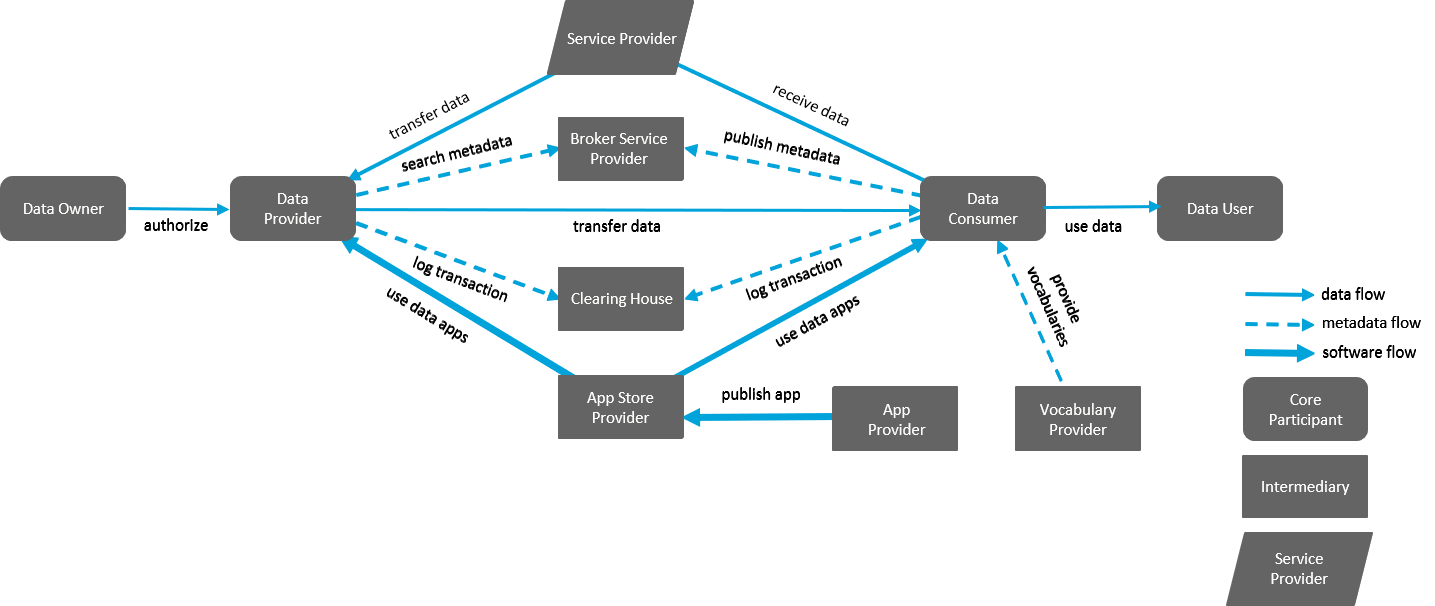
\includegraphics[width=6.53in,height=4.32in]{./media/image18.png}
		\caption{ Roles and interactions in the International Data Spaces}
		\label{fig:_Roles_and_interactions_in_the_International_Data_Spaces}
	\end{Center}
\end{figure}


%%%%%%%%%%%%%%%%%%%% Figure/Image No: 11 Ends here %%%%%%%%%%%%%%%%%%%%




\subsubsection{Digital Identities}
%\addcontentsline{toc}{subsubsection}{Digital Identities}

Establishing trust for data sharing and data exchange is a fundamental requirement. The IDS-RAM defines two basic types of trust: 1) Static Trust, based on the certification of participants and core technical components, and 2) Dynamic Trust, based on active monitoring of participants and core technical components. For data sharing and data exchange in the IDS, some preliminary actions and interactions are required. These are necessary for every participant, and involve the Certification Body, Evaluation Facilities, and the Dynamic Attribute Provisioning Service (DAPS). Figure \ref{fig:_Interactions_required_for_issuing_a_digital_identity_in_the_IDS} illustrates the roles and interactions required for issuing a digital identity in the IDS.  


%%%%%%%%%%%%%%%%%%%% Figure/Image No: 11 starts here %%%%%%%%%%%%%%%%%%%%

\begin{figure}[H]
	\begin{Center}
		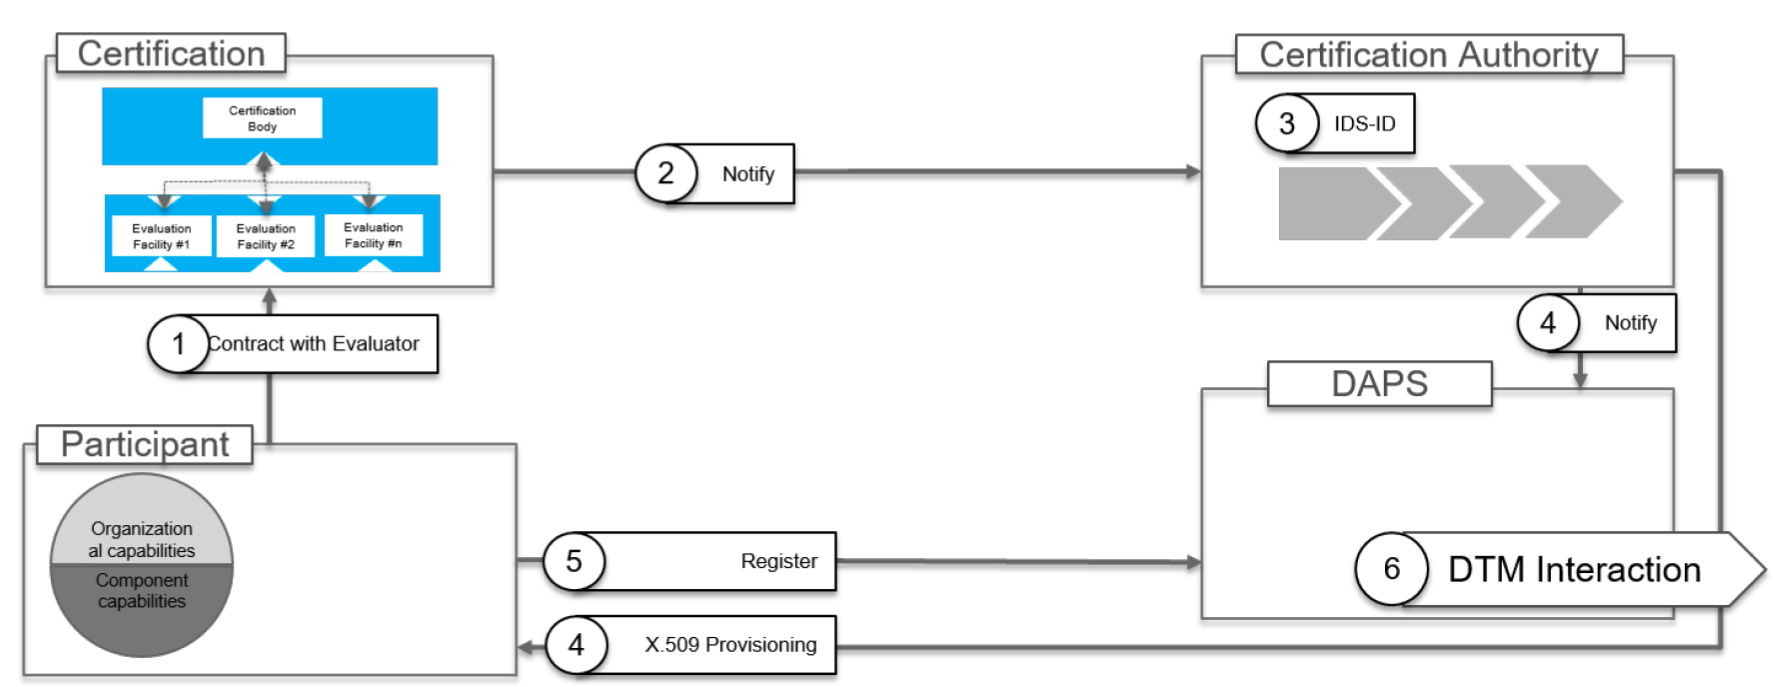
\includegraphics[width=6.53in,height=4.32in]{./media/DigitalIdentities.png}
		\caption{ Interactions required for issuing a digital identity in the IDS}
		\label{fig:_Interactions_required_for_issuing_a_digital_identity_in_the_IDS}
	\end{Center}
\end{figure}


%%%%%%%%%%%%%%%%%%%% Figure/Image No: 11 Ends here %%%%%%%%%%%%%%%%%%%%








\paragraph{Participant}
Certification is required for every participant and the majority of roles in the IDS, as defined above. Certification refers both to the organizational capabilities of the participant and the technical capabilities of the core technical components.


\paragraph{Certification} %ToDo: refer to section 4.2
Certification of a participant or core component involves the Certification Body and an Evaluation Facility (see section 4.2). Evaluation of a participant or a core component is executed upon request of the participant and relies on the contract between the participant and the Evaluation Facility. In the same way, a Service Provider can request evaluation of a component. In this process, the Certification Body is responsible for supervision of the Evaluation Facility involved.


\paragraph{Certification Authority} %ToDo: refer to sec 4.1
The Certification Authority is responsible for issuing, validating and revoking digital certificates (see section 4.1). A digital certificate is provided for a participant if both a valid certification for the participant and a valid certification for the core component is available. This means that the Certification Authority provides an IDS-ID for a combination of participant and core component. The digital certificate is valid not exceeding the validity of both certifications, participant certification and the certification of core component used by the participant. The Certification Authority provides the digital certificate to the participant upon request.


\paragraph{Dynamic Attribute Provisioning Service (DAPS)} %ToDo: referer
The information resulting from the certification process is passed on to the Dynamic Attribute Provisioning Service (DAPS). This includes master data and information on security profiles (see section 4.1.3.3.6 and Appendix B).  The CA provides the details on the digital certificate (public key and IDS-ID). The participant registers at the DAPS after successfully deploying the digital certificate inside the component.


\paragraph{Dynamic Trust Monitoring (DTM)}
Continuous monitoring of participants is necessary for classification of the trustworthiness of all participants in the ecosystem. Dynamic Trust Monitoring (DTM) implements a monitoring function for every IDS Component. The DTM shares information with the DAPS to notify each of the two participant in a data exchange transaction of the current level of trustworthiness of the other participant.


\paragraph{Interactions}
The roles described above interact with each other in a structured way, as described in Figure \ref{fig:_Interactions_required_for_issuing_a_digital_identity_in_the_IDS}. In the following, a brief description of these interactions is given (they are described in more detail in subsequent sections of the document): 


%\begin{enumerate}[label*={\fontsize{11pt}{11pt}\selectfont \arabic*.}]
\begin{enumerate}
	\item \textbf{Certification request:} This is a direct interaction between a participant and an evaluation facility to trigger an evaluation process based on IDS certification criteria.

	\item \textbf{Notification of successful certification:} The Certification Body notifies the Certification Authority of the successful certification of the participant and the core component. Validity of both certifications must be provided.

	\item \textbf{Generating the IDS-ID:} The CA generates a unique ID for the pair (participant and component) and issues a digital certificate (X.509).

	\item \textbf{Provisioning of X.509 Certificate:} The Certification Authority sends a digital certificate (X.509) to the participant in a secure and trustworthy way and notifies the DAPS.

	\item \textbf{Register:} After the digital certificate (X.509) is deployed inside the component, the component registers at the DAPS.

	\item \textbf{DTM Interaction}: The DTM and the DAPS exchange information on the behavior of the component, e.g. about security issues (vulnerabilities) or attempted attacks. 

\end{enumerate}




\subsubsection{Usage Contracts}
%\addcontentsline{toc}{subsubsection}{Usage Contracts}
A legally valid contract is the foundation of any business transaction. The IDS cannot, and does not intend to, replace legal contracts or licensing agreements. Instead, the IDS provides a technical framework for technically enforced agreements in addition to existing, legally binding contracts.

Many details of a business relationship cannot be modeled in machine-readable form. Nevertheless, the IDS specifies methods to define categories of applicable contracts, and it presents patterns to observe their usage and report validations. For this purpose, the IDS makes use of the Information Layer (see section 3.4). %ToDo:referer





%%%%%%%%%%%%%%%%%%%% Figure/Image No: 12 starts here %%%%%%%%%%%%%%%%%%%%

\begin{figure}[H]
	\begin{Center}
		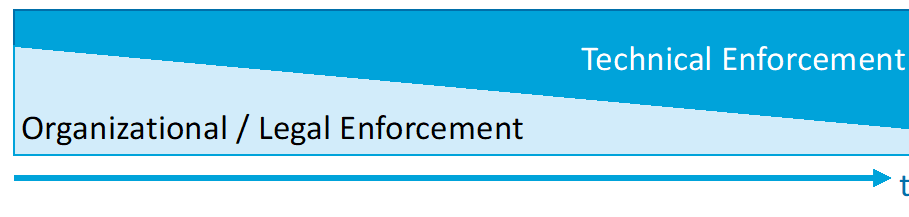
\includegraphics[width=6.53in,height=1.56in]{./media/image20_new.png}
		\caption{echnical Enforcement and organizational enforcement of usage policies}
		\label{fig:echnical_Enforcement_and_organizational_enforcement_of_usage_policies}
	\end{Center}
\end{figure}


%%%%%%%%%%%%%%%%%%%% Figure/Image No: 12 Ends here %%%%%%%%%%%%%%%%%%%%


%ToDo: referer
A Usage Contract comprises a set of Usage Policies. Each policy describes a certain permission or obligation of an IDS Resource (see section 3.4.3.2). Usage Contracts are written in a machine-readable format (according to the IDS Usage Policy Language, see section 3.4.4.1.1) and must be interpreted as defined in section 4.1.3.6. In any case, a Usage Contract must always be regarded as an extension of an existing legal agreement between two IDS participants, which can be overruled by them. As neither the IDS nor any other known technology stack can sufficiently interpret legal texts, any Usage Contract must always be in line with the concluded agreements. 
Each contract between IDS participants consists of a technical part and a non-technical part. The technical part focuses on the description of technical interfaces (Application Programming Interfaces) and the Usage Policy. Negotiation of the technical part of a contract must be supported by the Information Layer of the IDS-RAM. The non-technical part focuses on legal aspects of the intended data exchange. For automatic negotiation of contracts and conditions standard contracts are necessary (but not yet available today). 

%%%%%%%%%%%%%%%%%%

\subsection{Functional Layer}
\label{sec_functional_layer}
%\addcontentsline{toc}{subsection}{Functional Layer}
The Functional Layer defines –  irrespective of existing technologies and applications –  the functional requirements of the International Data Spaces, and the features to be implemented resulting thereof.



%%%%%%%%%%%%%%%%%%%% Figure/Image No: 13 starts here %%%%%%%%%%%%%%%%%%%%

\begin{figure}[H]
	\begin{Center}
		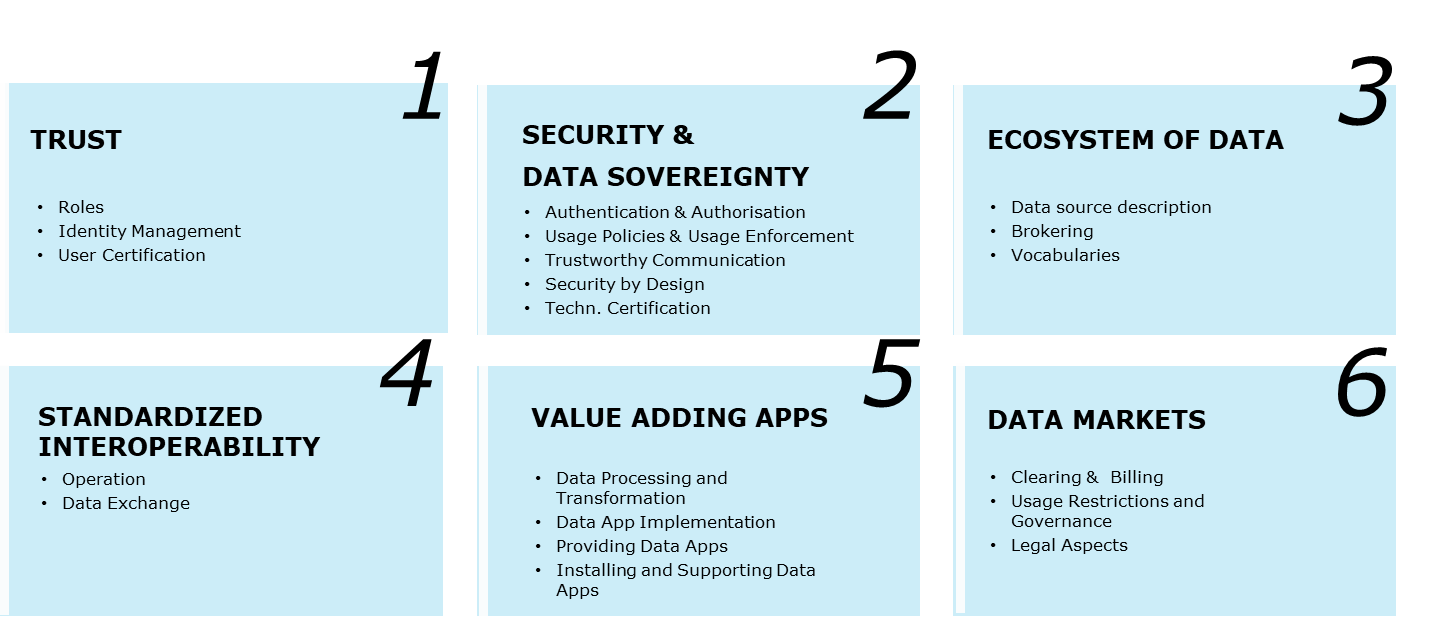
\includegraphics[width=6.44in,height=2.78in]{./media/image21.png}
		\caption{ Functional architecture of the International Data Spaces}
		\label{fig:_Functional_architecture_of_the_International_Data_Spaces}
	\end{Center}
\end{figure}


%%%%%%%%%%%%%%%%%%%% Figure/Image No: 13 Ends here %%%%%%%%%%%%%%%%%%%%


Figure \ref{fig:_Functional_architecture_of_the_International_Data_Spaces} shows the functional architecture of the International Data Spaces, subdividing the requirements into six groups of software functionality to be provided by the IDS. These six groups comply with the strategic requirements outlined in Section \ref{subsec:Goals_of_IDS}.



 The following subsections give a brief summary of these functional requirements. The full list of functional requirements can be found in a separate document entitled $``$Functional Overview$"$ .

\subsubsection{Trust}\label{subsec:functional_layer_trust}
%\addcontentsline{toc}{subsubsection}{Trust}

Although requirements related to trust are usually non-functional, they are addressed by the Functional Layer, since they represent fundamental features of the International Data Spaces. The $``$Trust$"$  group comprises three main aspects (roles, identity management, and user certification), which are complemented by governance aspects (see Section 4.3). %ToDo referer

\paragraph{Roles\\}
Each role in the International Data Spaces has certain rights and duties. For example, the Identity Provider is responsible for offering services to create, maintain, manage, monitor, and validate identity information of and for participants in the International Data Spaces. More information about the roles is given in Section 3.1. %ToDo: referer


\paragraph{Identity Management\\}
Every Connector participating in the International Data Spaces must have a unique identifier and a valid certificate. In addition, each Connector must be able to verify the identity of other Connectors (with special conditions being applied here; e.g., security profiles). 

\paragraph{User Certification\\}
Each participant in the International Data Spaces must undergo certification in order to establish trust among all participants. More information about the certification process is given in Section 4.2. %ToDo referer


\subsubsection{Security and Data Sovereignty}
%\addcontentsline{toc}{subsubsection}{Security and Data Sovereignty}
Like requirements related to trust, requirements related to security and data sovereignty are also usually non-functional, but are still addressed by the Functional Layer, since they represent fundamental features of the International Data Spaces. The $``$Security and data sovereignty$"$  group contains four major aspects: authentication $\&$  authorization; usage policies $\&$  usage enforcement; trustworthy communication $\&$  security by design; and technical certification.


\paragraph{Authentication $\&$  Authorization\\}
Each Connector must have a valid X.509 certificate. With the help of this certificate, each participant in the International Data Spaces that operates an endpoint is able to verify the identity of any other participant. Certain conditions (e.g. security profiles) may also apply here. More information about authentication is given in Section 4.1. % ToDo:referer

The Connector serving as the data source must be able to verify the receiving Connector’s capabilities and security features as well as its identity. More information about authorization is given in Section 4.1. %ToDo referer

\paragraph{Usage Policies $\&$  Usage Enforcement\\}
In the IDS, Data Owners and Data Providers can always be sure their data is handled by a Data Consumer according to the usage policies specified. Each participant can define usage policies and attach them to outbound data. Policies might include restrictions, such as disallowing persistence of data, or disallowing transfer of data to other parties, for example. More information about usage policies and usage enforcement is given in Section 4.1. % ToDo referer

\paragraph{Trustworthy Communication $\&$  Security by Design\\}
Connectors, App Stores, and Brokers can check if the Connector of the connecting party is running a trusted (i.e. certified) software stack. Any communication between (external) Connectors can be encrypted and integrity protected. Each Data Owner and Data Provider must be able to ensure that their data is handled by the Connector of the Data Consumer according to the usage policies specified: otherwise the data will not be sent. To reduce the impact of compromised applications, appropriate technical measures must be applied (e.g. isolating Data Apps from each other and from the Connector). Data Providers and Data Consumers can decide about the level of security to be applied for their respective Connectors by deploying Connectors supporting the selected security profile. More information about trustworthy communication and security by design is given in Section 4.1. %ToDo referer


\paragraph{Technical Certification\\}
The core components of the International Data Spaces, and especially the Connectors, require certification from the Certification Body in order to establish trust among all participants. More information about technical certification is given in Section 4.2. %ToDo referer


\subsubsection{Ecosystem of Data}
%\addcontentsline{toc}{subsubsection}{Ecosystem of Data}
Being able to describe, find and correctly interpret data is another key aspect of the International Data Spaces. Therefore, every data source in the International Data Spaces is described on the Information Layer (see section 3.4). % ToDo referer

The $``$Ecosystem of Data$"$  group comprises three major aspects: data source description, brokering, and vocabularies.


\paragraph{Data Source Description\\}
Participants must have the opportunity to describe, publish, maintain and manage different versions of metadata. Metadata should describe the syntax and serialization as well as the semantics of data sources. Furthermore, metadata should describe the application domain of the data source. The operator of a Connector must be able to define the price, the pricing model, and the usage policies regarding certain data. More information about data source description is given in Section 3.4. %ToDo referer


\paragraph{Brokering\\}
The operator of a Connector must be able to provide an interface for data and metadata access. Each Connector must be able to transmit metadata of its data sources to one or more brokers. Each participant must be able to browse and search metadata in the metadata repository, provided the participant has the right to access the metadata. Furthermore, each participant must be able to browse the list of participants registered at a broker. More information about brokering is given in Section 3.5.2. %ToDo referer


\paragraph{Vocabularies\\}
To create and structure metadata, the operator of a Connector may use vocabularies. In doing so, an operator of a Connector can use existing vocabularies, create own vocabularies, or work with other operators on new vocabularies provided by vocabulary hubs. Vocabulary hubs are central servers that store vocabularies and enable collaboration. Collaboration may comprise search, selection, matching, updating, requests for changes, version management, deletion, duplicate identification, and unused vocabularies. Vocabulary hubs need to be managed. More information about vocabularies is given in Section 3.4.%ToDo referer


\subsubsection{Standardized Interoperability}
%\addcontentsline{toc}{subsubsection}{Standardized Interoperability}
Standardized data exchange between participants is the fundamental aspect of the International Data Spaces. The IDS Connector is the main technical component for this purpose.

\paragraph{Operation\\}
Participants should be able to run the Connector software in their own IT environment. Alternatively, they can run a Connector on mobile or embedded devices. The operator of the Connector must be able to define the data workflow inside the Connector. Users of the Connector must be identifiable and manageable. Passwords and key storage must be protected. Every action, data access, data transmission, incident, etc. should be logged. Using this logging data, it should be possible to draw up statistical evaluations on data usage etc. Notifications about incidents should be sent automatically.


\paragraph{Data Exchange\\}
The Connector must receive data from an enterprise backend system, either through a push-mechanism or a pull-mechanism. The data can be provided via an interface or pushed directly to other participants. To do so, each Connector must be uniquely identifiable. Other Connectors can subscribe to data sources or pull data from these sources. Data can be written into the backend system of other participants.


\subsubsection{Value Adding Apps}
%\addcontentsline{toc}{subsubsection}{Value Adding Apps}
Before or after the actual data exchange, data may need to be processed or transformed. For this purpose, the International Data Spaces offers Data Apps. Each Data App has a lifecycle, spanning its implementation, provision in the App Store, installation, and support. The App Store should therefore be clearly visible and recognizable to every participant.

\paragraph{Data Processing and Transformation\\}
A data processing app (which is a subtype of a Data App) should provide a single, clearly defined processing function to be applied on input data for producing an expected output. A data transformation app (also a subtype of a Data App) should be able to transform data from an input format into a different output format in order to comply with the requirements of the Data Consumer (without any substantial change made to the information contained in the data; i.e., loss-less transformation). 

\paragraph{Data App Implementation\\}
The developers of Data Apps should be able to annotate the software with metadata (about functions and interfaces, pricing models, licenses, etc.). Data Apps must explicitly define their interfaces, dependencies, and access requirements.


\paragraph{Providing Data Apps\\}
Any authorized Data App developer can initiate a software provision process (App Store publication). Prior to publication in the App Store, Data Apps must pass an optional evaluation and certification process controlled by the Certification Body. The App Store should support authorized users in their search for a suitable application in an adequate fashion. Access of privileged users (e.g., administrators or operators) should require strong authentication (e.g., 2-factor authentication).


\paragraph{Installing and Supporting Data Apps\\}
A dedicated Connector service should support authorized users in (un-)installing Data Apps not originating from an official App Store. In addition, it should support authorized users in searching, installing, and managing (e.g., removal or automated updates) Data Apps retrieved from an App Store.


\subsubsection{Data Markets}
%\addcontentsline{toc}{subsubsection}{Data Markets}
Data to be exchanged in the International Data Spaces may have monetary value. Therefore, the International Data Spaces has to integrate data market concepts, like clearing and billing, but also governance.

\paragraph{Clearing $\&$  Billing\\}
The Data Owner can define the pricing model (e.g. pay per transfer, pay per access, pay per day/month/year), and the price of data. Any transaction of any participant can be logged. The clearing and billing process must be simple and standardized.


\paragraph{Usage restrictions, and governance\\}
Governance in the International Data Spaces comprises five aspects: data as an economic good, data ownership, data sovereignty, data quality, and data provenance. More information about governance is given in Section 4.3. %ToDO referer

\paragraph{Legal aspects\\}
Trading data on a data marketplace requires legal contracts and conditions that can be negotiated in an automated way. Therefore, standard contracts for typical data exchange transactions are necessary.  
